% Implementation 
\chapter{Implementation}
\label{sec:implement}

This section provides a brief overview of the experimental setup and aims to motivate the choice of datasets, libraries and frameworks.

\section{Scope and Limitations}
\label{sec:implement:scope}
% Here an overview of what was implemented and what was left out and why 




\section{Experimental Setup}
\label{sec:implement:setup}
% Gather, scatter in tensorflow 
Usually neighbourhood relationships between nodes are represented with adjacency matrices. In this paper, however we choose to work with adjacency lists, as it brings some benefits. Since the experiments are conducted on \ac{ogb} datasets, where adjacency is represented as a list, we make use of tensorflow's tensorflow~\cite{tensorflow} gather and scatter operations.

% Description gather, scatter 
gather fetches data at the indexed locations and scatter updates the output data at the indexed loacations. This is used to realize the convolution

% Formula --> Code 
% Implementation of regularization techniques 



% HERE ABOUT DESCREPANCY BETWEEN PAPER AND CODE ! --> cite github for seed paper 


\subsection{Choice of Frameworks}
\label{sec:implement:setup:choice}
Below we give a quick overview of used daasets and frameworks and motivate the choice.


\subsubsection{Datasets}
\label{sec:implement:setup:choice:data}
% Datasets - OGB 
Despite the fact, that machine learning on graph structured data is carried out in many areas and has many interesting use cases ranging from social networks, to molecular graphs, to manifolds, to source code~\cite{Hu2020},
there does not exist and unified framework for working with graph-structured data. Furthermore commonly-used datasets and evaluation procedures suffer from multiple issues, that negatively affect the quality of predictions and the reliability of evaluations of models.
Machine learning algorithms rely heavily on data. In order for a \ac{gnn} to be able to make accurate predictions, there is need for a sufficient amount of properly prepared training data. To be able to compare different models against each other there is need of standardized splitting and evaluation methods.

% Problems overview 
Today, most of the frequently-used
graph datasets are extremely small compared to graphs found in
real applications. Same datasets, such as Cora, CiteSeer and PubMed are used again and again to train various models leading to poor scalability in the majority of cases. Small datasets also make it hard to rigorously evaluate data-hungry models, such as \acfp{gnn}. The performance of a \ac{gnn} on these datasets is often unstable and nearly statistically identical to each other, due to the small number of samples the models are trained and evaluated on~\cite{Kipf2017,Xu2019, Hu2020}.

% OGB benefits  
\textbf{\Ac{ogb}} offers a wide range of different-sized graph-datasets from different domains for a variety of different classification tasks and provides an unified pipeline for working with the datasets in \ac{ml} tasks.
The unified experimental protocol with standardized dataset splits, evaluation metrics and cross-validation protocols makes it easy to compare perfromance reported across various studies~\cite{Hu2020}.

% overview of standardized pipeline 
% graphic ? 
Working with \ac{ogb} consists of following steps:

\begin{enumerate}
    \item \Ac{ogb} provides realistic, different-scaled graph benchmark datasets that cover different prediction tasks, are from diverse application.
    \item Dataset processing and splitting is fully automated. \Ac{ogb} data loaders automatically download and process graphs and further split the datasets in a standardized manner. This is compatible with multiple libraries and a library-agnostic option is also provided.
    \item This step includes developing an \ac{ml} model to train on the ogb datasets.
    \item  \Ac{ogb} evaluates the model in a dataset-dependent manner, and outputs the model performance appropriate for the task at hand.
    \item \Ac{ogb} provides public leaderboards to keep track of recent advances.
\end{enumerate}

\begin{figure}[H]
    \centering
    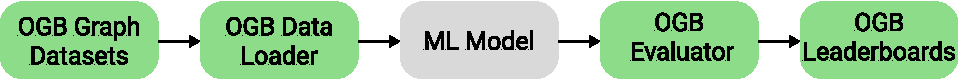
\includegraphics[width= 0.90\linewidth]{gfx/implementation/OGB_pipeline}
    \caption{\textbf{Overview of the standardized OGB pipeline} adapted from \cite{Hu2020}}\label{fig:implement:pipeline}
\end{figure}
% Agnostic choica av. 
% ----------------------------------------------------------------------------
% Choice of metrics for my tasks 

% Node classification 

% Node regression 

% Graph classification 

% Graph regression 
%-----------------------------------------------------------------------------

% Introduction of MAD 
\subsubsection{Metrics}
\label{sec:implement:setup:choice:metrics}
To be able to make systematic and quantative statements about the positive effects on oversmoothing by using different regularization techniques, one has to be able to monitor the smoothness of nodes at different execution steps during training. Therefore, a choice of a suitable metric is of great importance, as it helps to access the extent of the effect produced by various regularization techniques and compare them against each other in terms of efficacy.
% TODO: CITE

\textbf{\Ac{mad}} ~\cite{Chen2020} is a metric for smoothness, the similarity of graph nodes representations. In that sence over-smoothness is the similarity of nodes representations among different classes.
While smoothing to some extent is desired(we assume spatial similarity between nodes), mixing features of nodes with different lables over several iterations leads to oversmoothing.

It is therefore important to differentiate between different types of messages between nodes. Signal/information is the messaging of nodes, which share the same class/label, i.e., intra-class communication and noize denotes intra-class comunication. Having too many inter-class edges leads to much noise by encorporating messages from other classes, which results in oversmoothing.

Because of that it is crucial to have a measure of the quality of the recieved messages. A way to do that is to consider the information-to noise ratio i.e., the fraction of intra-class node pairs and all node pairs that have interaction trough \ac{gnn} model. That way it is possible to differentiate between remote and neihbouring nodes and calculate the \textbf{\ac{madg}}, which is strongly positive correlated with a models accuracy.

% Formal definition 
\ac{mad} is calculated as follows:

Given the graph representation matrix $H \in \mathbb{R}^{n \times h}$ we
first obtain the distance matrix $D \in \mathbb{R}^{n \times n}$ for $H$ by
computing the cosine distance between each node pair.

\begin{align*}
    D_{i,j} = 1 - \frac{H_{i,:} \cdot H_{j,:}}{\mid H_{i,:}\mid  \cdot \mid H_{j,:}\mid} \; \;  i,j \in [1,2, \dots, n],
\end{align*}

where $H_{k}$ is the $k$-th row of $H$. The reason to use cosine distance is that cosine distance is not affected by the absolute value of the node vector,
thus better reflecting the smoothness of graph representation. Then we filter the target node pairs by element-wise mutliplication $D$ with a mask matrix $M^{tgt}$

\begin{align*}
    D^{tgt} = D \odot M^{tgt},
\end{align*}
where $\odot$ denotes the element-wise mutliplication: $M^{tgt} \in \{0,1\}^{n \times n}; M_{i,j}^{tgt}= 1$ only if node pair $(i,j)$ is the target one.
Next we access the average distance $\bar{D}^{tgt}$ for non-zero values along each row in $D^{tgt}:$

\begin{align*}
    \bar{D}_{t}^{tgt} = \frac{\sum_{j=0}^{n}D_{i,j}^{tgt}}{\sum_{j=0}^{n}\mathds{1}(D_{i,j}^{tgt})}
\end{align*}

% Intuition behind all this 

\Ac{mad} gives acess to the smoothness of a node and pairs of nodes troughout iterations, which makes it easy to "track down" oversmoothing.

% graphic signal/ information & noise 